\documentclass[a4paper,oneside,14pt]{extreport}

\usepackage[T2A]{fontenc}
\usepackage[utf8]{inputenc}
\usepackage[english,russian]{babel}

\usepackage[left=30mm, right=10mm, top=20mm, bottom=20mm, bindingoffset=0cm]{geometry}

\usepackage{microtype}
\usepackage{tikz}

\usepackage{setspace}
\onehalfspacing
\usepackage{graphicx}
\usepackage{indentfirst}
\setlength{\parindent}{12.5mm}

\usepackage{titlesec}
\titleformat{\chapter}{\LARGE\bfseries}{\thechapter}{10pt}{\LARGE\bfseries}
\titlespacing*{\chapter}{0pt}{-20pt}{10pt}
\titleformat{\section}{\large\bfseries}{\thesection}{10pt}{\large\bfseries}
\titlespacing*{\section}{0pt}{0pt}{10pt}
\titleformat{\subsection}{\normalsize\bfseries}{\thesubsection}{10pt}{\normalsize\bfseries}
\titlespacing*{\subsection}{0pt}{5pt}{5pt}

\addto{\caption}{\renewcommand*{\contentsname}{Содержание}}
\usepackage[square,sort,comma,numbers]{natbib}
\renewcommand{\bibsection}{\chapter*{Список литературы}}

\usepackage{caption}

\usepackage{wrapfig}
\usepackage{float}
\usepackage{listings}
\usepackage{graphicx}
\graphicspath{{.}}
\newcommand{\imgwc}[4]
{
	\begin{figure}[#1]
		\center{\includegraphics[width=#2]{inc/img/#3}}
		\caption{#4}
		\label{img:#3}
	\end{figure}
}
\newcommand{\imghc}[4]
{
	\begin{figure}[#1]
		\center{\includegraphics[height=#2]{inc/img/#3}}
		\caption{#4}
		\label{img:#3}
	\end{figure}
}
\newcommand{\imgsc}[4]
{
	\begin{figure}[#1]
		\center{\includegraphics[scale=#2]{inc/img/#3}}
		\caption{#4}
		\label{img:#3}
	\end{figure}
}

\usepackage{pgfplots}
\pgfplotsset{compat=newest}

\usepackage{listings}
\usepackage{listingsutf8}
\lstset{
	basicstyle=\footnotesize\ttfamily,
	keywordstyle=\color{blue},
	stringstyle=\color{red},
	commentstyle=\color{gray},
	numbers=left,
	numberstyle=\tiny,
	numbersep=5pt,
	frame=false,
	breaklines=true,
	breakatwhitespace=true,
	inputencoding=utf8/koi8-r
}

\newcommand{\code}[1]{\texttt{#1}}

\usepackage{amsmath}
\usepackage{mathtools}
\usepackage{amssymb}

\usepackage[unicode]{hyperref}
\hypersetup{hidelinks}

\makeatletter
\newcommand{\vhrulefill}[1]
{
	\leavevmode\leaders\hrule\@height#1\hfill \kern\z@
}
\makeatother


\begin{document}
	\pagenumbering{Alph}
\documentclass[../report.tex]{subfiles}
\graphicspath{{\subfix{../images/}}}

\begin{document}
\thispagestyle{empty}
\doublespacing
\noindent
\begin{minipage}[l]{0.15\textwidth}
	\centering
	
\includegraphics{bmstu_low}
\end{minipage}
% нельзя делать пустую строку
\begin{minipage}[r]{0.85\textwidth}
	\centering\bfseries\singlespacing
	Министерство науки и высшего образования Российской Федерации\\
Федеральное государственное бюджетное образовательное учреждение\\
высшего образования\\
«Московский государственный технический университет\\
имени Н.Э. Баумана\\
(национальный исследовательский университет)»\\
(МГТУ им. Н.Э. Баумана)
\end{minipage}

\vspace*{5mm}
\noindent
\rule{\textwidth}{3pt}

\noindent
\MakeUppercase{Факультет}
\underline{«Информатика и системы управления»}

\noindent
\MakeUppercase{Кафедра}
\underline{«Программное обеспечение ЭВМ и информационные технологии»}

\vspace*{4cm}

\noindent
\center{
\textbf{
\MakeUppercase{Отчет\\
о лабораторной работе №5
}\\
\MakeUppercase{Конвеерная обработка данных}\\
по дисциплине:\\
«Анализ алгоритмов»
}}

\vspace*{3cm}

\begin{FlushLeft}
Руководитель: ст. преп. каф. ИУ7 \noindent\underline{\makebox[3em][l]{}} Волкова Л.Л.\\
Исполнитель: студ. гр. ИУ7-55Б \noindent\underline{\makebox[3em][l]{}} Муравьев И.А.
\end{FlushLeft}

\vspace*{\fill}
\center{
Москва 2021
}


\end{document}
\pagenumbering{arabic}
\newpage
\tableofcontents
\lstset{
	language = python,
	basicstyle=\small\sffamily,
	numbers=left,
	numberstyle=\tiny,
	stepnumber=1,
	numbersep=5pt,
	xleftmargin =.19in,
	showspaces=false,
	showstringspaces=false,
	showtabs=false,
	frame=single,
	tabsize=2,
	captionpos=t,
	breaklines=true,
	breakatwhitespace=false,
	escapeinside={\#*}{*)}
}

\newpage

\addcontentsline{toc}{chapter}{Введение}
\chapter*{Введение}
\textbf{Цель:} сравнить трудоемкость сортировок выбором, шейкерной и Шелла.

\textbf{Задачи:}
\begin{enumerate}
	\item Изучить алгоритмы сортировки перемешиванием, выбором и Шелла.
	\item Вычислить и сравнить трудоемкость реализуемых алгоритмов на основе выбранной модели вычислений.
	\item Реализовать и протестировать алгоритмы:
	\begin{enumerate}
		\item шейкерной сортировки;
		\item сортировки выбором;
		\item сортировки Шелла.
	\end{enumerate}
	\item Провести сравнительный анализ алгоритмов по затрачиваемым ресурсам (процессорному времени работы).
\end{enumerate}
\newpage

\chapter{Аналитическая часть}
Алгоритмы сортировки — это алгоритмы, которые берут некоторую последовательность из n элементов $a_1, a_2,..., a_n$ и переставляют элементы таким образом, чтобы получившаяся последовательность $a'_1,a'_2,...,a'_n$ удовлетворяла условию: $a'_1 \leqslant a'_2 \leqslant ... \leqslant a'_n$ \cite{SortAlgorithms}.

Алгоритмы сортировки можно классифицировать по:
\begin{itemize}
	\item принципу сортировки:
	\begin{itemize}
		\item сортировки, использующие сравнения: быстрая сортировка, пирамидальная сортировка, сортировка вставками и другие;
		\item сортировки, не использующие сравнения: блочная сортировка, поразрядная сортировка, сортировка подсчётом и другие;
		\item прочие, например, обезьянья сортировка;
	\end{itemize}
	\item устойчивости (сортировка является устойчивой в том случае, если для любой пары элементов с одинаковым ключами, она не меняет их порядок в отсортированном списке);
	\item вычислительной сложности;
	\item использованию дополнительной памяти;
	\item рекурсивности;
	\item параллельности;
	\item адаптивности (сортировка является адаптивной в том случае, когда она выигрывает от того, что входные данные могут быть частично или полностью отсортированы, например, сортировка вставками);
	\item использованию внутренней или внешней памяти компьютера. 
\end{itemize}

\section{Шейкерная сортировка}
Шейкерная сортировка (двунаправленная, перемешиванием) - оптимизированный алгоритм пузырьковой сортировки. В основе данной сортировки лежит сравнение двух элементов, которое осуществляется в двух направлениях поочередно, постепенно сужая диапазон сортировки. В итоге за один проход в конец массива “всплывает” максимальный элемент из диапазона, а за следующий проход — в начало массива минимальный (мы рассматриваем сортировку по возрастанию). Эти элементы можно больше не рассматривать и таким образом диапазон сужается с двух сторон. \cite{Shaker}.

Изначальная версия алгоритма подразумевает изменение границы на единицу каждый раз вне зависимости от наличия упорядоченных промежутков в массиве, таким образом цикл повторяется много раз даже для упорядоченных частей массива. В связи с этим существует оптимизация в виде добавления переменной, запоминающей место последнего обмена при перестановке элементов, а затем смещения соответствующей границы на полученное значение.

В данной работе рассматривается классическая реализация алгоритма сортировки перемешиванием.

\section{Сортировка выбором}
Сортировка выбором работает следующим образом: на каждом проходе выбирается минимальный элемент и смещается в начало. При этом каждый новый проход начинается со сдвигом вправо, то есть первый проход начинается с первого элемента, второй проход — со второго \cite{Selection}.

\section{Сортировка Шелла}
Сортировка Шелла может рассматриваться в качестве обобщения как сортировки пузырьком, так и сортировки вставками.

Идея метода заключается в сравнении разделенных на группы элементов последовательности, находящихся друг от друга на некотором расстоянии. Изначально это расстояние равно d или N/2, где N — общее число элементов. На первом шаге каждая группа включает в себя два элемента расположенных друг от друга на расстоянии N/2; они сравниваются между собой, и, в случае необходимости, меняются местами. На последующих шагах также происходят проверка и обмен, но расстояние d сокращается на d/2, и количество групп, соответственно, уменьшается. Постепенно расстояние между элементами уменьшается, и на d=1 проход по массиву происходит в последний раз \cite{Shell}.

\section{Вывод}
Были рассмотрены алгоритмы сортировки перемешиванием, выбором и Шелла. Все сортировки являются простыми, но отличаются подходом: шейкерная проходит массив в двух направлениях, сравнивая и обменивая соседние элементы, сортировка Шелла сравнивает и обменивает элементы с некоторым шагом, сортировка выбором на каждом проходе ищет минимальный элемент и сдвигает его в начало.

\newpage
\chapter{Конструкторская часть}
Данный раздел содержит схемы алгоритмов сортировки, реализуемых в работе (Шелла, шейкерной, выбором), а также теоретические вычисления трудоемкости для каждого из них.

\section{Требования к программному обеспечению}
Требования, выдвигаемые к разрабатываемому ПО:
\begin{itemize}
	\item входные данные - последовательность вещественных чисел для сортировки;
	\item выходные данные - отсортированная последовательность, лежащая в области памяти исходного массива.
\end{itemize}

\section{Схемы алгоритмов}
В данном пункте раздела представлены схемы реализуемых в работе алгоритмов.

\subsection{Схема алгоритма шейкерной сортировки}
На рисунке \ref{fig:Shaker} представлена схема алгоритма сортировки перемешиванием.

\begin{figure}[H]
	\centering
	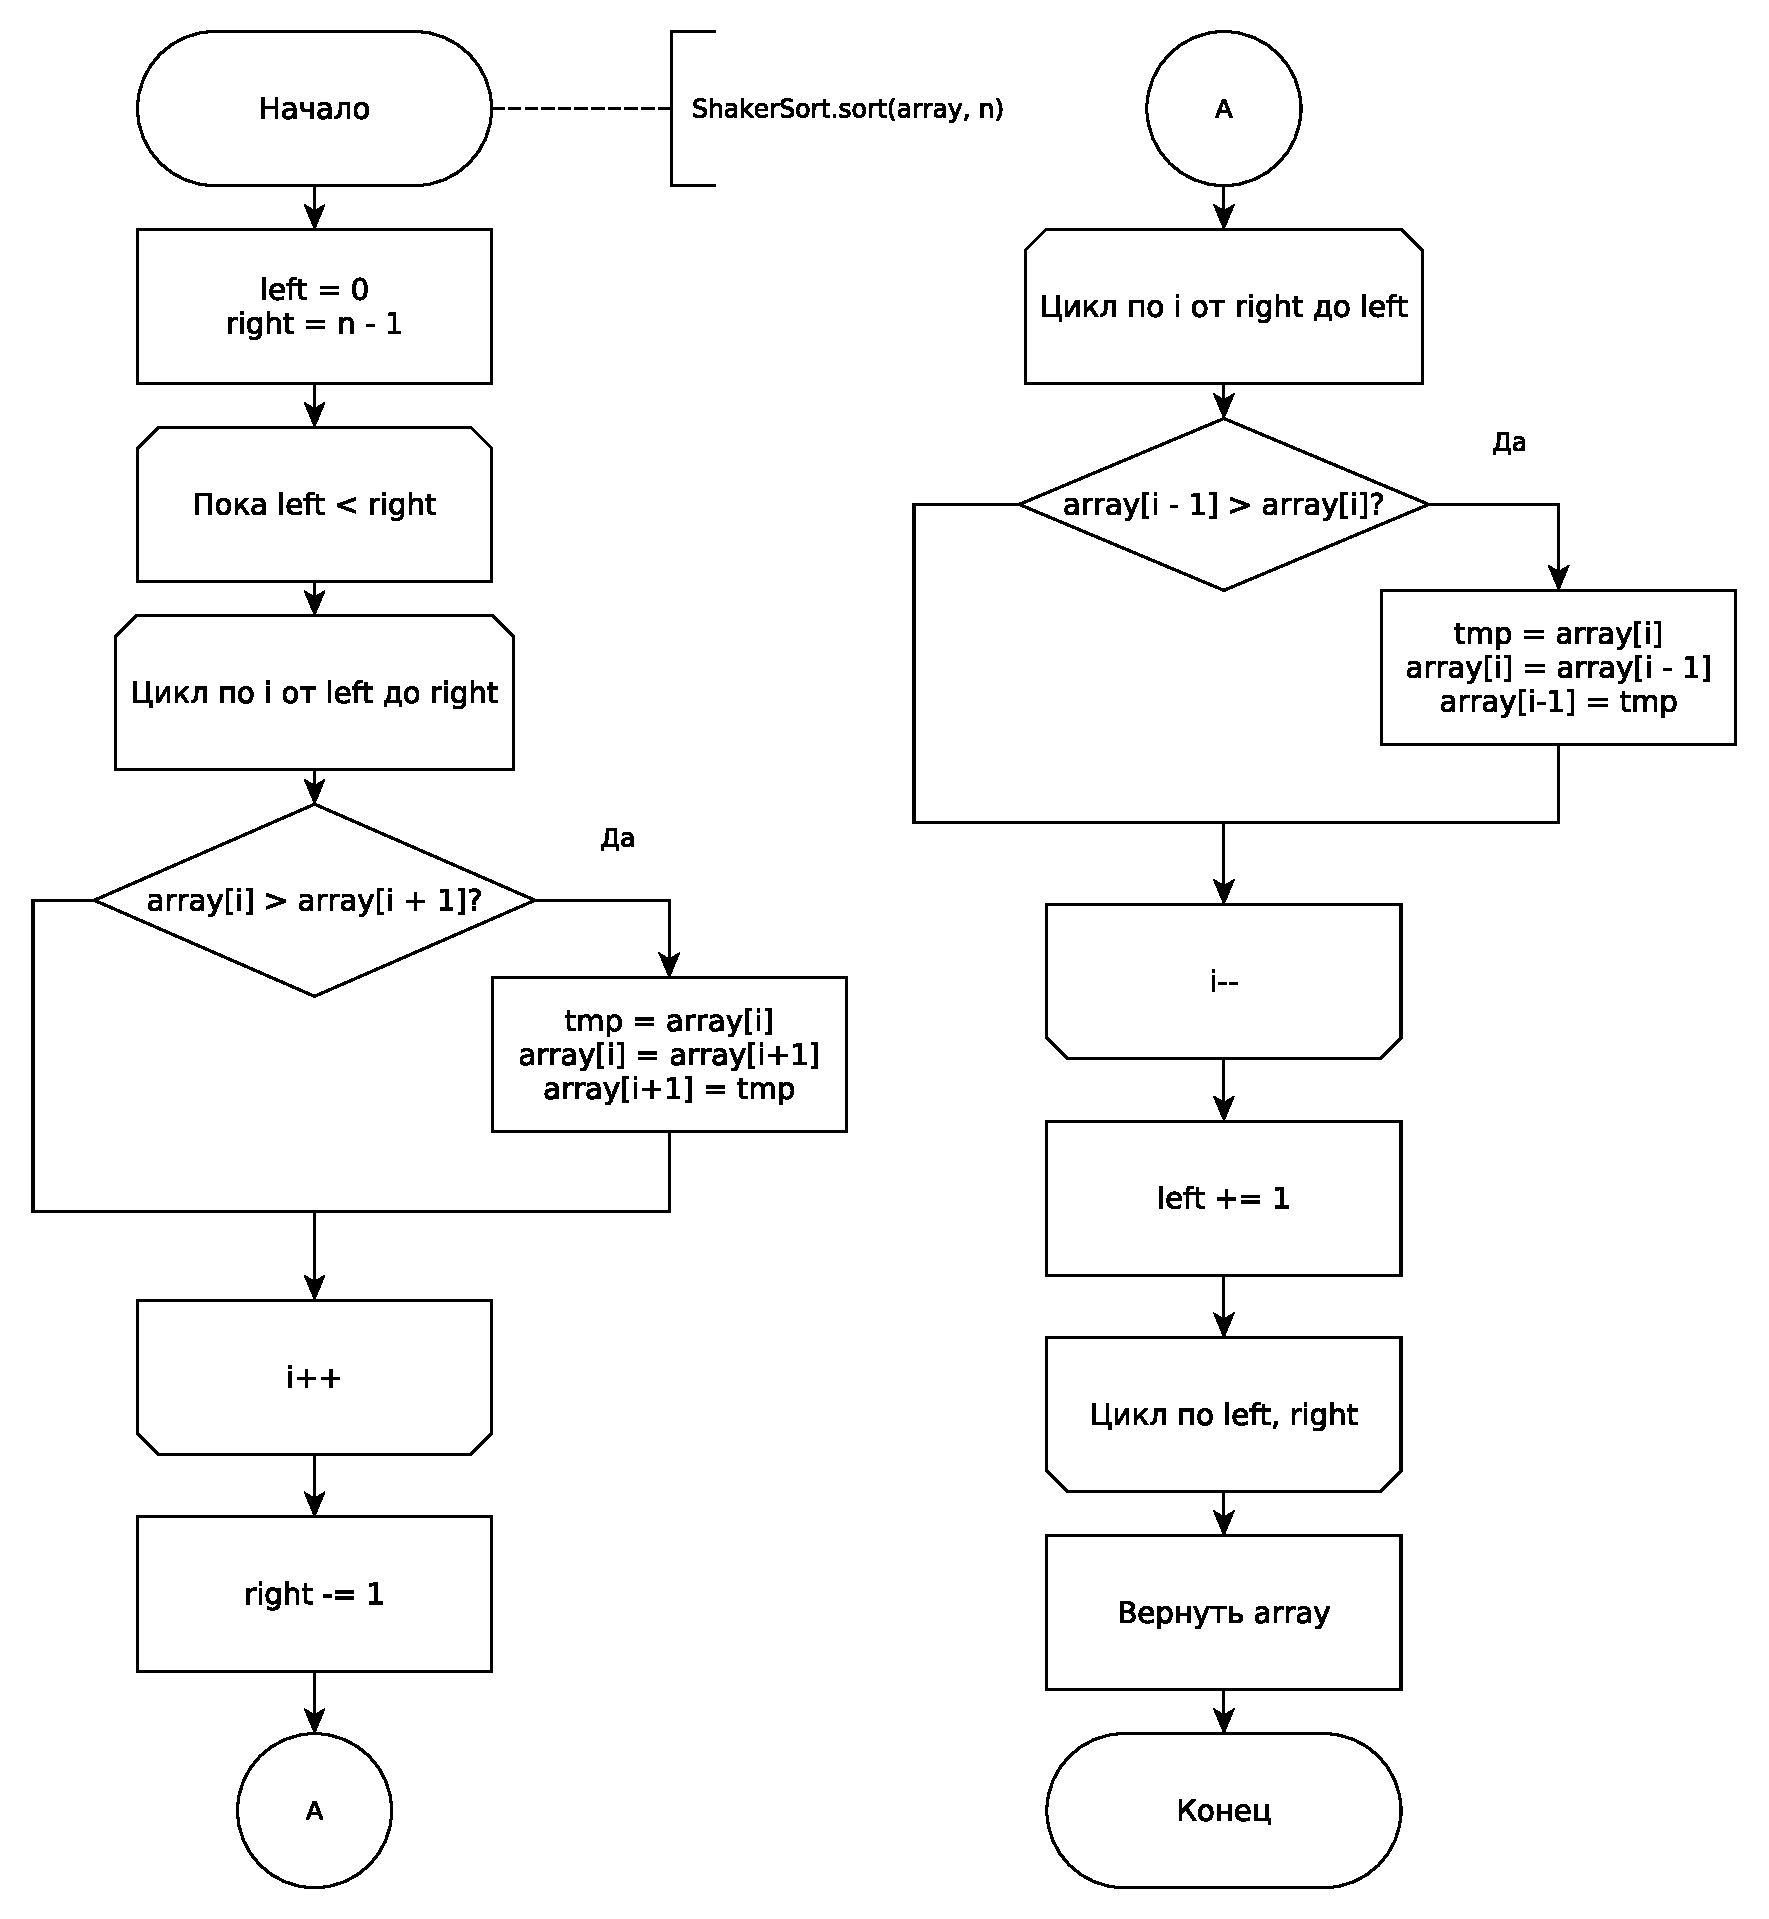
\includegraphics[width=1.01\linewidth]{images/ShakerSort}
	\caption{Схема алгоритма шейкерной сортировки}
	\label{fig:Shaker}
\end{figure}

\subsection{Схема алгоритма сортировки выбором}
На рисунке \ref{fig:Selection} представлена схема алгоритма сортировки выбором.

\captionsetup{justification=centering, singlelinecheck=false}

\begin{figure}[H]
	\centering
	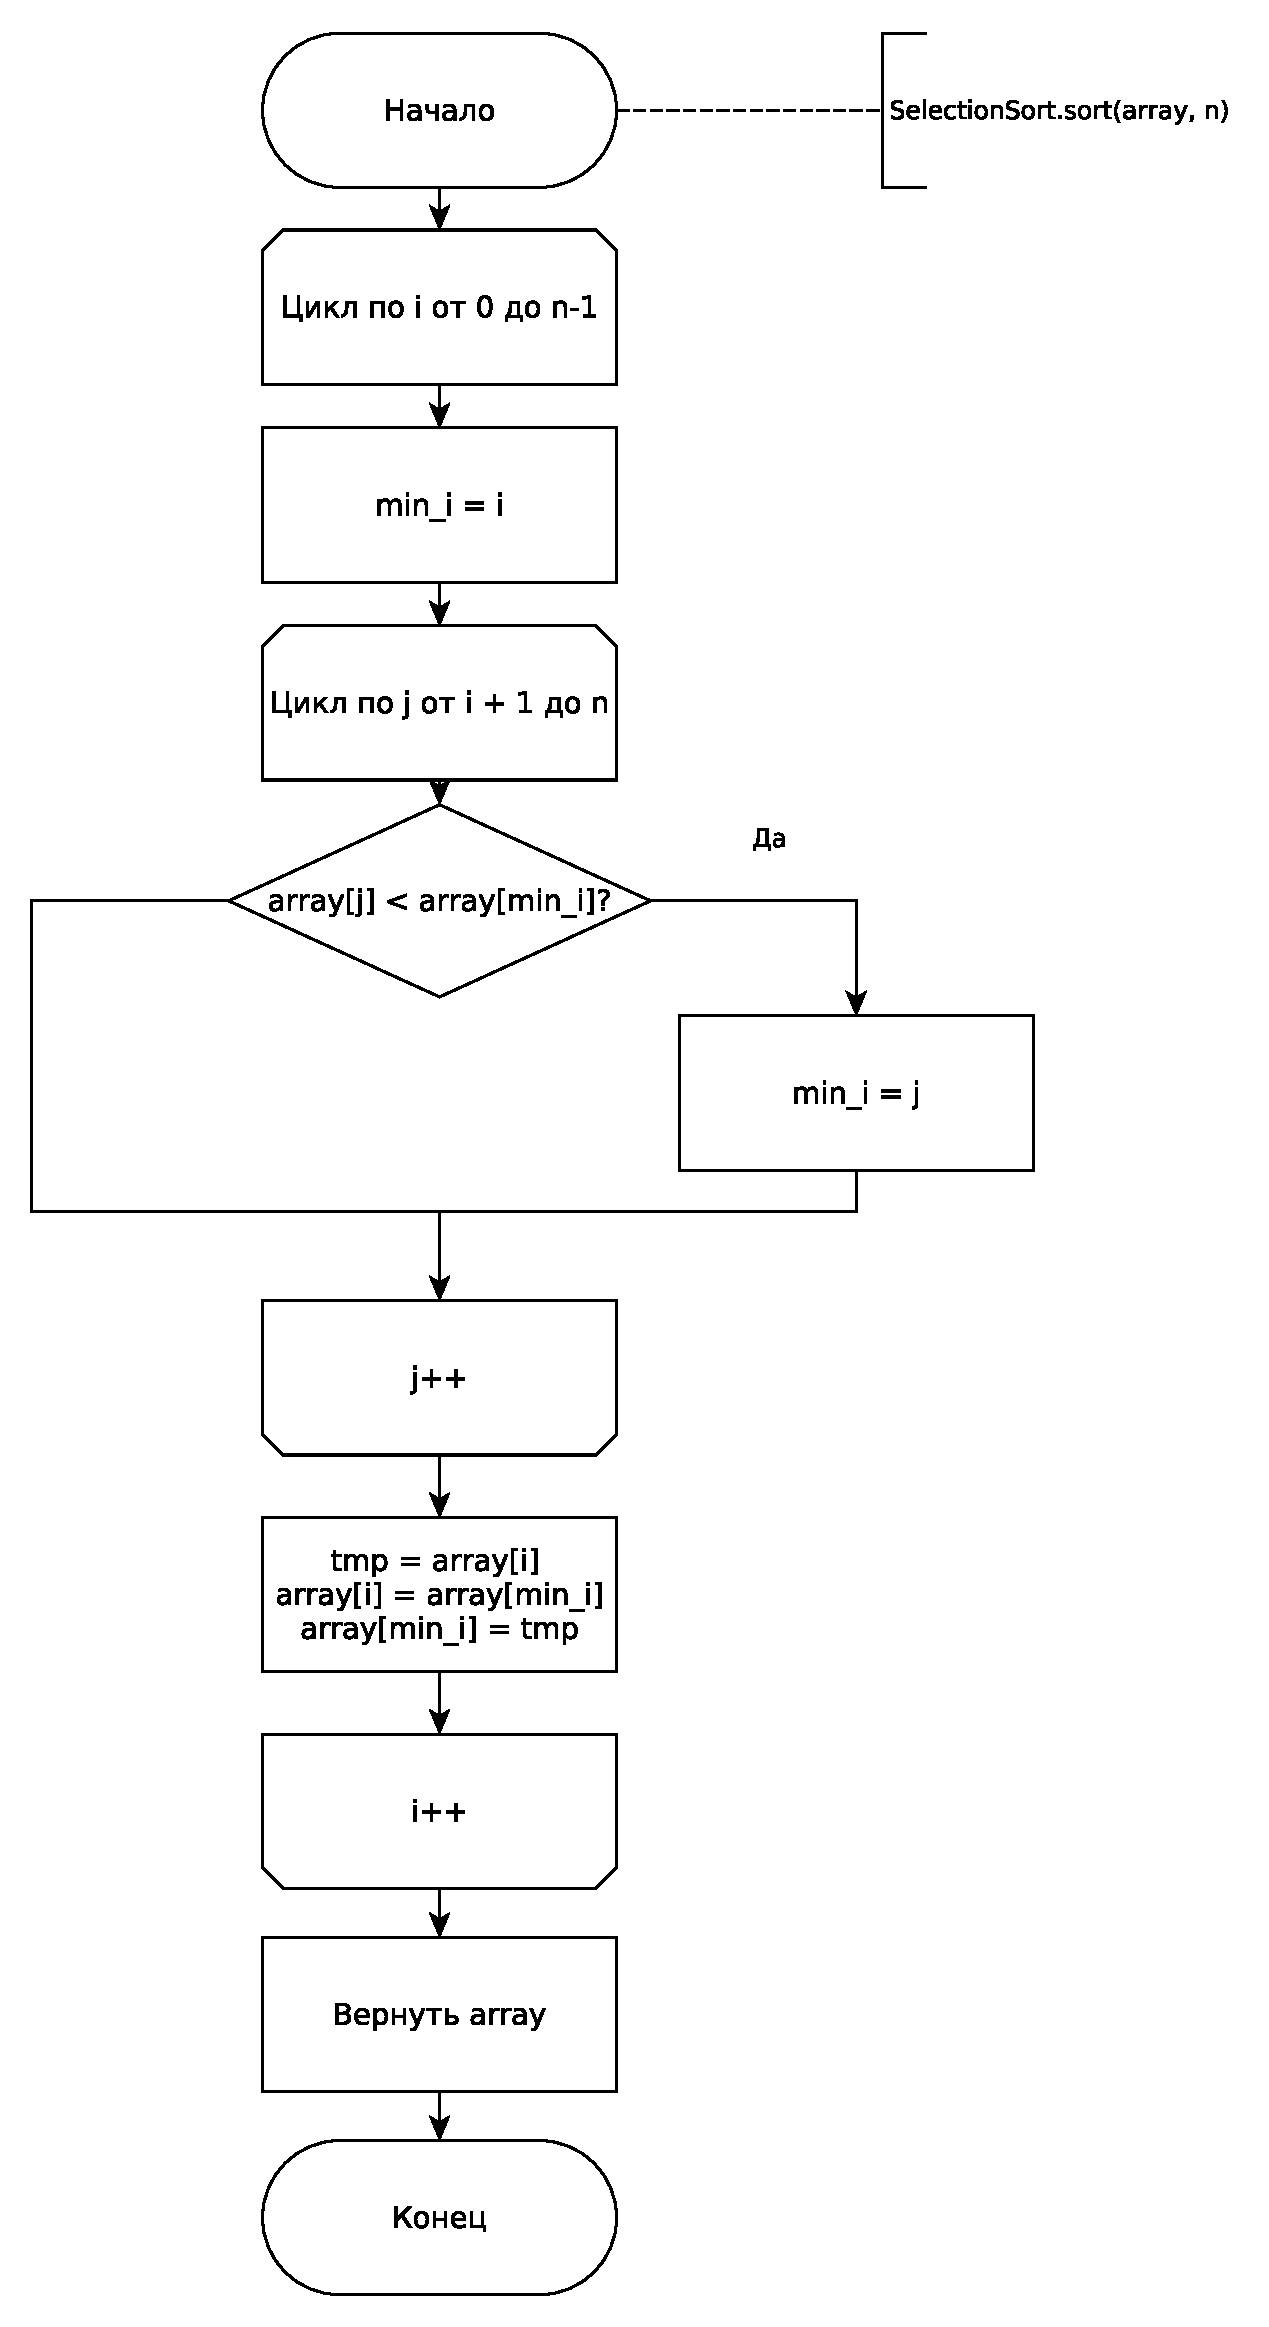
\includegraphics[width=0.8\linewidth]{images/SelectionSort}
	\caption{Схема алгоритма сортировки выбором}
	\label{fig:Selection}
\end{figure}

\subsection{Схема алгоритма сортировки Шелла}
Схема алгоритма сортировки Шелла представлена на рисунке \ref{fig:Shell}.

\begin{figure}[H]
	\centering
	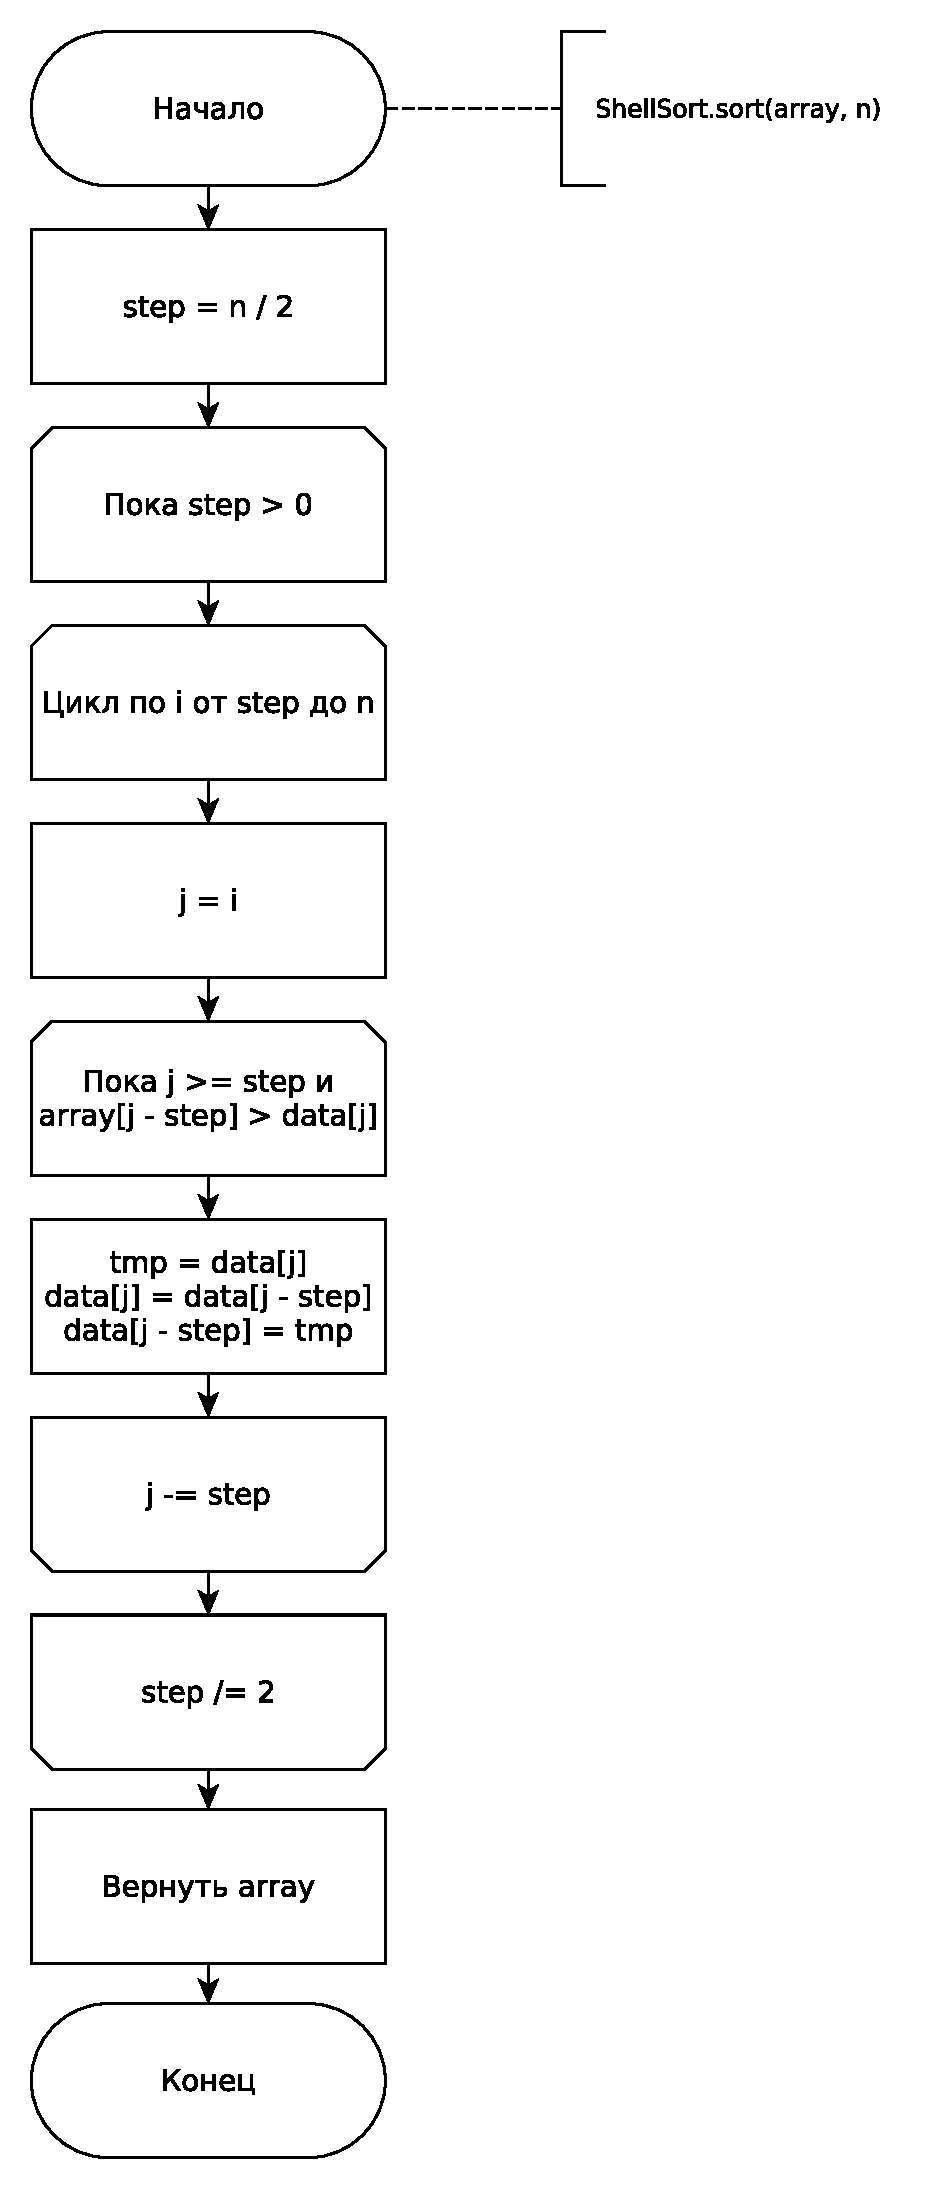
\includegraphics[width=0.62\linewidth]{images/ShellSort}
	\caption{Схема сортировки Шелла}
	\label{fig:Shell}
\end{figure}

\section{Модель вычислений}
В данной работе используется следующая модель вычислений для определения трудоемкости алгоритмов \cite{ulanov}:
\begin{itemize}
	\item операции из списка \ref{eq:op_1} имеют трудоемкость 1;
	\begin{equation} \label{eq:op_1}
	+, -, +=, -=, =, ==, !=, !, \&\&, ||, <, >, <<, >>, <=, >=, [] 
	\end{equation}
	\item операции из списка \ref{eq:op_2} имеют трудоемкость 2;
	\begin{equation} \label{eq:op_2}
	*, /, //, \%, *=, /=
	\end{equation}
	\item трудоемкость цикла рассчитывается по формуле \ref{eq:for};
	\begin{equation} \label{eq:for}
	\begin{array}{ll}
		f_{\text{цикла for}} = f_{\text{инициализации}} + f_{\text{сравнения}} +\\
		N_{\text{итераций}} (f_{\text{тела}} + f_{\text{инкремента}} + f_{\text{сравнения}})
	\end{array}
	\end{equation}
	\item трудоемкость условного оператора if ($
	\begin{array}{ll}
	if (\text{условие}) \ then \ \{A\}\ else \	 \{B\}  
	\end{array}
	$) рассчитывается по формуле \ref{eq:if_cnt} с учетом того, что трудоемкость условного перехода равна 0. \\
	\begin{equation} \label{eq:if_cnt}
	f_{if} = f_{\text{условия}} +
	\begin{cases}
	min(f_A, f_B), & \textrm{лучший случай}\\
	max(f_A, f_B), & \textrm{худший случай}
	\end{cases}
	\end{equation}
\end{itemize}

\section{Трудоемкость алгоритмов сортировки}
В данном подразделе представлены расчеты трудоемкости для алгоритмов..
\subsection{Трудоемкость шейкерной сортировки}
Трудоемкость алгоритма сортировки перемешиванием складывается из следующих частей:
\begin{itemize}
	\item затраты на содержание внешнего цикла от 1 до n - 1 с шагом 2: $f_{\text{внеш}}=1 + 2 + 1 + \frac{n}{2}(1 + 2 + f_{forw} + f_{back}) = 4 + \frac{n}{2}(3 + f_{init forw} + f_{init back})$;
	\item инициализация вложенного цикла, проходящего массив в прямом направлении: $f_{init forw}=2$;
	\item инициализация вложенного цикла, проходящего массив в обратном направлении: $f_{init back}=2$;
	\item внутренний цикл, проходящий массив в прямом направлении: $f_{forward}= \frac{1 + n - 1}{2} \cdot \frac{n}{2}(1 + 1 + 4 + f_{\text{усл}}) = \frac{n^2}{4} (6 + f{\text{усл}})$;
	\item внутренний цикл, проходящий массив в обратном направлении: $f_{back}= \frac{1 + n - 2}{2} \cdot \frac{n-1}{2}(1 + 1 + 4 + f_{\text{усл}}) = \frac{(n-1)^2}{4} (6 + f_{\text{усл}})$;
	\item тело условия (худший случай): $f_{\text{усл}} = 2 + 4 + 2 = 9$
\end{itemize}

Подставив полученные выражения, для лучшего случая (отсортированный массив) получим формулу \ref{eq:shaker_best}, для худшего (отсортированный в обратном порядке) - выражение \ref{eq:shaker_worst}.
\begin{equation} \label{eq:shaker_best}
\begin{array}{ll}
f = 4 + \frac{n}{2}(3 + 2 + 2) + \frac{n^2}{4} (6 + 0) + \frac{(n-1)^2}{4} (6 + 0) =\\ 3n^2 + \frac{n}{2} + \frac{11}{2} \approx 3n^2
\end{array}
\end{equation}
\begin{equation} \label{eq:shaker_worst}
\begin{array}{ll}
f = 4 + \frac{n}{2}(3 + 2 + 2) + \frac{n^2}{4} (6 + 9) + \frac{(n-1)^2}{4} (6 + 9) =\\ \frac{15}{2}n^2 - 4n + \frac{31}{4} \approx \frac{15}{2}n^2
\end{array}
\end{equation}


\subsection{Трудоемкость алгоритма сортировки выбором}
Трудоемкость алгоритма сортировки выбором содержит следующие части:
\begin{itemize}
	\item внешний цикл от 1 до n: $f_i = 1 + 1 + (n - 1)\cdot(1 + 1 + 1 + f_{swap} + f_{init\ j}) = 2 + (n - 1)\cdot(3 + f_{swap} + f_{init\ j})$;
	\item затраты на инициализацию внутреннего цикла: $f_{init\ j} = 2 + 1 = 3$;
	\item внутренний цикл от i + 1 до n: $f_j = \frac{1 + n - 1}{2} \cdot (n -1) (1 + 1 + 3 + f_{\text{усл}}) = \frac{n^2 - n}{2} \cdot(5 + f_{\text{усл}})$; 
	\item тело условия (худший случай): $f_{\text{усл}} = 1$;
	\item трудоемкость операции обмена: $f_{swap} = 2 + 4 + 2 = 9$.
\end{itemize}

Таким образом, для лучшего случая (отсортированный массив) получим выражение \ref{eq:selection_best}.
\begin{equation} \label{eq:selection_best}
\begin{array}{ll}
f = 2 + (n - 1)\cdot(3 + 9 + 3) + \frac{n^2 - n}{2} \cdot(5 + 0) = \frac{5}{2} n^2 + \frac{25}{2}n^2 - 13 \approx \frac{5}{2}n^2
\end{array}
\end{equation}

Для худшего случая (отсортированный в обратном порядке массив) получим выражение \ref{eq:selection_worst}.
\begin{equation} \label{eq:selection_worst}
\begin{array}{ll}
f = 2 + (n - 1)\cdot(3 + 9 + 3) + \frac{n^2 - n}{2} \cdot(5 + 1) = 3n^2 + 12n - 13 \approx 3n^2
\end{array}
\end{equation}

\subsection{Трудоемкость сортировки Шелла}
Для определения трудоемкости сортировки Шелла воспользуемся данными ресурсов. Таким образом, трудоемкость лучшего случая (массив отсортирован в правильном порядке) составляет $n\log n$, худшего (неподходящий выбор шагов сравнения) - $n^2$ \cite{ShellEff}.

\section{Вывод}
В данном разделе на основе приведенных в аналитическом разделе теоретических данных были составлены схемы алгоритмов для реализации в технологической части, вычислена трудоемкость лучшего и худшего случаев алгоритмов сортировок перемешиванием и выбором, приведены данные трудоемкости алгоритма сортировки Шелла. Лучший случай для выбранных алгоритмов оказался общим, это случай обработки отсортированного массива. Худший случай совпал для шейкерной сортировки и сортировки выбором, это обработка отсортированного в обратном порядке массива. Худшим случаем для алгоритма сортировки Шелла является случай неудачного выбора шага сравнения. Приблизительная трудоемкость шейкерной сортировки для лучшего случая равна $3n^2$, худшего - $\frac{15}{2}n^2$; сортировки выбором для лучшего случая - $\frac{5}{2}n^2$, для худшего - $3n^2$; сортировки Шелла для лучшего случая - $n \log n$, для худшего случая - $n^2$. Таким образом, наиболее эффективной является сортировка Шелла, наименее - шейкерная сортировка.
\newpage

\chapter{Технологическая часть}
Данный раздел содержит обоснование выбора языка и среды разработки, реализацию алгоритмов.

\section{Средства реализации}
Для реализации программы был выбран язык программирования Python~\cite{python}. Такой выбор обусловлен следующими причинами:
\begin{itemize}
	\item имеется большой опыт разработки;
	\item имеет большое количество расширений и библиотек, что облегчает работу с некоторыми типами данных и математическими формулами;
	\item обладает информативной документацией.
\end{itemize}

\section{Реализация алгоритмов}
В листингах \ref{lst:Shaker} - \ref{lst:Shell} представлены реализации рассматриваемых алгоритмов.
\newpage
\captionsetup{singlelinecheck=false, justification=raggedright}
\begin{lstlisting}[caption=Шейкерная сортировка, label={lst:Shaker}]
class ShakerSort(Sort):
	def __init__(self):
		super(ShakerSort, self).__init__()
	
	def sort(self, array):
		left = 0
		right = len(array) - 1
		
		while left < right:
			for i in range(left, right):
				if array[i] > array[i + 1]:
					array[i], array[i + 1] = array[i + 1], array[i]
					right -= 1
			
			for i in range(right, left, -1):
				if array[i - 1] > array[i]:
					array[i], array[i - 1] = array[i - 1], array[i]
					left += 1
		return array
\end{lstlisting}

\begin{lstlisting}[caption=Сортировка выбором, label={lst:Select}]
class SelectionSort(Sort):
	def __init__(self):
		super(SelectionSort, self).__init__()
	
	def sort(self, array):
		n = len(array)
		for i in range(n - 1):
			min_i = i
			for j in range(i + 1, n):
				if array[j] < array[min_i]:
					min_i = j
			array[i], array[min_i] = array[min_i], array[i]
		return array
\end{lstlisting}
\newpage
\begin{lstlisting}[caption=Сортировка Шелла, label={lst:Shell}]
class ShellSort(Sort):
	def __init__(self):
		super(ShellSort, self).__init__()
		
	def sort(self, array):
		n = len(array)
		step = n // 2
		while step > 0:
			for i in range(step, n):
				j = i
				while j >= step and array[j - step] > array[j]:
					array[j - step], array[j] = array[j], array[j - step]
					j -= step
			step //= 2
		return array
\end{lstlisting}

\section{Тестирование}
В таблице \ref{tab:tests} представлены использованные для тестирования методом "черного ящика"\ данные, были рассмотрены все возможные тестовые случаи. Все тесты пройдены успешно. Здесь и далее "Массив" - входная последовательность, "Шейкерная" - алгоритм шейкерной сортировки, "Выбором" - алгоритм сортировки выбором, "Шелла" - алгоритм сортировки Шелла.

\begin{table}[H]
	\begin{center}
		\captionsetup{justification=raggedleft, singlelinecheck=false}
		\caption[]{\label{tab:tests} Проведенные тесты}

	\begin{tabular}{|c|c|c|c|}
		\hline
		\rule[-1ex]{0pt}{2.5ex} Массив & Шейкерная & Выбором & Шелла \\
		\hline
		\rule[-1ex]{0pt}{2.5ex} [1, 2, 3, 4, 5, 6] & [1, 2, 3, 4, 5, 6] & [1, 2, 3, 4, 5, 6] & [1, 2, 3, 4, 5, 6] \\
		\hline
		\rule[-1ex]{0pt}{2.5ex} [6, 5, 4, 3] & [3, 4, 5, 6] & [3, 4, 5, 6] & [3, 4, 5, 6] \\
		\hline
		\rule[-1ex]{0pt}{2.5ex} [-1, 1, 2, 0, 3, -2]  & [-2, -1, 0, 1, 2, 3] & [-2, -1, 0, 1, 2, 3] & [-2, -1, 0, 1, 2, 3] \\
		\hline
		\rule[-1ex]{0pt}{2.5ex} [-2, 3, -2, 6, 3, 1] & [-2, -2, 1, 3, 3, 6] & [-2, -2, 1, 3, 3, 6] & [-2, -2, 1, 3, 3, 6] \\
		\hline
		\rule[-1ex]{0pt}{2.5ex} [2] & [2] & [2] & [2] \\
		\hline
		\rule[-1ex]{0pt}{2.5ex} [5, 6, -9, 3, -10] & [-10, -9, 3, 5, 6] & [-10, -9, 3, 5, 6] & [-10, -9, 3, 5, 6] \\
		\hline
		\rule[-1ex]{0pt}{2.5ex} [] & Ошибка & Ошибка & Ошибка \\
		\hline
		
	\end{tabular}
\end{center}
\end{table}
\section{Выводы}
В данном разделе были реализованы и протестированы алгоритмы сортировки: перемешиванием, выбором и Шелла.
\newpage

\chapter{Экспериментальная часть}
В данном разделе сравниваются реализованные алгоритмы, дается сравнительная оценка затрат и время.

\section{Пример работы программы}
Пример работы программы представлен на рисунке \ref{fig:work_example}.
\captionsetup{singlelinecheck=true}
\begin{figure}[H]
	\centering
	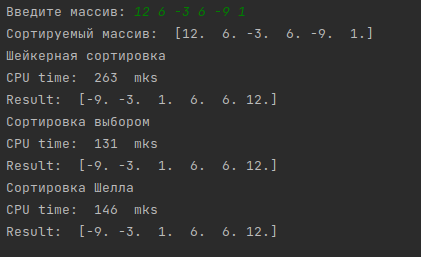
\includegraphics[width=0.7\linewidth]{images/example}
	\caption{Пример работы программы}
	\label{fig:work_example}
\end{figure}

\section{Технические характеристики}
Технические характеристики устройства, на котором выполнялось исследование:
\begin{itemize}
	\item операционная система: Ubuntu 20.01 Linux x86\_64~\cite{ubuntu};
	\item оперативная память: 8 Гб;
	\item процессор: AMD Ryzen5 3500U~\cite{processor}.
\end{itemize}

\section{Время выполнения алгоритмов}
Время выполнения алгоритмов замерялось на автоматически генерируемых массивах необходимого размера и упорядоченности (вещественные числа находятся в диапазоне [-n x 10, n x 10]) с использованием функции getrusage библиотеки resources~\cite{resource}. Усредненные результаты замеров процессорного времени приведены в таблицах ниже.

На рисунке \ref{fig:random_arrays} представлен график зависимости времени работы алгоритмов от размера произвольно упорядоченных массивов на основе таблицы \ref{tab:rand_time}. Для произвольно упорядоченных массивов самым эффективным алгоритмом оказался алгоритм Шелла. Выигрыш сортировки Шелла по сравнению с алгоритмом сортировки выбором составляет от 1.5 до 16 раз; по сравнению с шейкерной сортировкой - от 2 до 30 раз. Выигрыш по времени увеличивается с увеличением размера входной последовательности. Наименее эффективной оказалась шейкерная сортировка, которая проигрывает сортировке выбором в среднем в 2 раза. 
\begin{table}[H]
	\begin{center}
		\captionsetup{justification=raggedleft, singlelinecheck=false}
		\caption{\label{tab:rand_time} Время обработки произвольных массивов разной длины в микросекундах}
		\begin{tabular}{|c c c c|} 
			\hline
			Размер&Шейкер&Выбором&Шелла\\ [0.5ex]
			\hline
			5 &  96 &  71 &  66\\ 
			\hline
			7 &  150 &  116 &  106\\ 
			\hline
			10 &  290 &  207 &  185\\ 
			\hline
			20 &  1092 &  690 &  498\\ 
			\hline
			50 &  6713 &  3824 &  1904\\ 
			\hline
			100 &  26545 &  14576 &  4982\\ 
			\hline
			200 &  104361 &  56225 &  12367\\ 
			\hline
			500 &  616529 &  212110 &  22072\\ 
			\hline
			1000 &  1584832 &  841228 &  53035\\ 
			\hline
		\end{tabular}
	\end{center}
\end{table}

\begin{figure}[H]
	\centering
	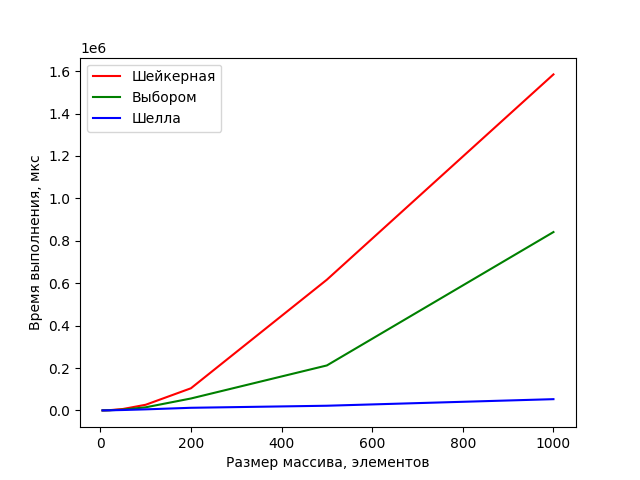
\includegraphics[width=0.9\linewidth]{images/rand_arrays}
	\caption{Зависимость времени работы алгоритмов сортировки от размера произвольно упорядоченного массива}
	\label{fig:random_arrays}
\end{figure}

На рисунке \ref{fig:sort_arrays} представлен график зависимости времени работы алгоритмов от размера упорядоченных массивов на основе таблицы \ref{tab:sort_time}. Для упорядоченных массивов самым эффективным алгоритмом также оказался алгоритм Шелла. Его выигрыш по сравнению с другими сортировками составил от 2 до 56 раз, при увеличении с увеличением размера входной последовательности. Время работы алгоритмов сортировки перемешиванием и выбором на упорядоченных массивах почти совпало с незначительным преимуществом сортировки выбором.

\begin{table}[H]
	\begin{center}
		\captionsetup{justification=raggedleft, singlelinecheck=false}
		\caption{\label{tab:sort_time} Время обработки упорядоченных массивов разной длины в микросекундах}
		\begin{tabular}{|c c c c|} 
			\hline
			Размер&Шейкер&Выбором&Шелла\\ [0.5ex]
			\hline
			5 &  86 &  74 &  43\\ 
			\hline
			7 &  103 &  126 &  53\\ 
			\hline
			10 &  181 &  210 &  97\\ 
			\hline
			20 &  665 &  693 &  234\\ 
			\hline
			50 &  3833 &  3820 &  709\\ 
			\hline
			100 &  14827 &  14389 &  1679\\ 
			\hline
			200 &  57329 &  55620 &  4004\\ 
			\hline
			500 &  355309 &  327702 &  7988\\ 
			\hline
			1000 &  890107 &  866875 &  16047\\ 
			\hline
		\end{tabular}
	\end{center}
\end{table}

\begin{figure}[H]
	\centering
	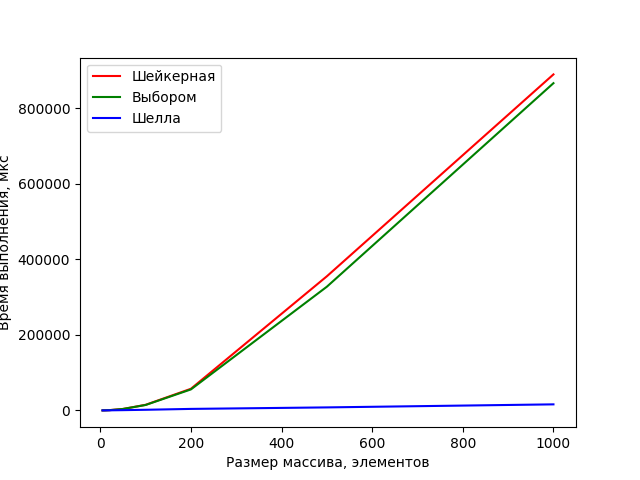
\includegraphics[width=1\linewidth]{images/sorted_arrays}
	\caption{Зависимость времени работы алгоритмов сортировки от размера упорядоченного массива}
	\label{fig:sort_arrays}
\end{figure}

На рисунке \ref{fig:reverse_arrays} представлен график зависимости времени работы алгоритмов от размера упорядоченных в обратном порядке массивов на основе таблицы \ref{tab:kontr_time}. В данном случае также  самым эффективным алгоритмом оказался алгоритм Шелла. Его выигрыш по сравнению с сортировкой выбором составил от 2 до 22 раз, однако на небольших массивах размером до 10 элементов выигрыш незначителен. Наименее эффективным алгоритмом сортировки оказался алгоритм шейкерной сортировки, который работает в 2-3 раза дольше сортировки выбором и от 2 до 60 раз дольше сортировки Шелла.
\begin{table}[H]
	\begin{center}
		\captionsetup{justification=raggedleft, singlelinecheck=false}
		\caption{\label{tab:kontr_time} Время обработки упорядоченных в обратном порядке массивов разной длины в микросекундах}
		\begin{tabular}{|c c c c|} 
			\hline
			Размер&Шейкер&Выбором&Шелла\\ [0.5ex]
			\hline
			5 &  105 &  73 &  68\\ 
			\hline
			7 &  201 &  121 &  101\\ 
			\hline
			10 &  390 &  209 &  182\\ 
			\hline
			20 &  1522 &  681 &  474\\ 
			\hline
			50 &  9328 &  3803 &  1424\\ 
			\hline
			100 &  37057 &  14492 &  3531\\ 
			\hline
			200 &  144316 &  55750 &  8540\\ 
			\hline
			500 &  737375 &  221832 &  16998\\ 
			\hline
			1000 &  2278427 &  818325 &  37704\\ 
			\hline
		\end{tabular}
	\end{center}
\end{table}

\begin{figure}[H]
	\centering
	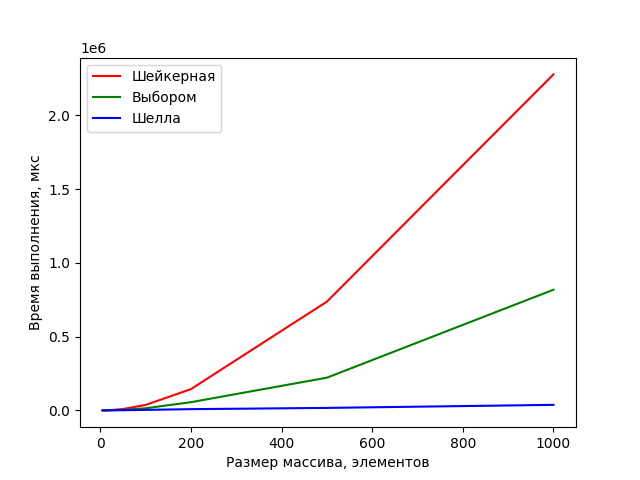
\includegraphics[width=1\linewidth]{images/reverse_arrays}
	\caption{Зависимость времени работы алгоритмов сортировки от размера упорядоченного в порядке убывания массива}
	\label{fig:reverse_arrays}
\end{figure}

На рисунках \ref{fig:shaker_gr} - \ref{fig:shell_gr} представлены зависимости работы алгоритмов сортировок от размера и упорядоченности входного массива. Худшим случаем для алгоритма сортировки Шелла оказался произвольно упорядоченный массив, что говорит о неудачно выбранном шаге сравнения элементов для итераций. Время работы алгоритма сортировки выбором практически одинаковое для лучшего и худшего случаев.

\begin{figure}[H]
	\centering
	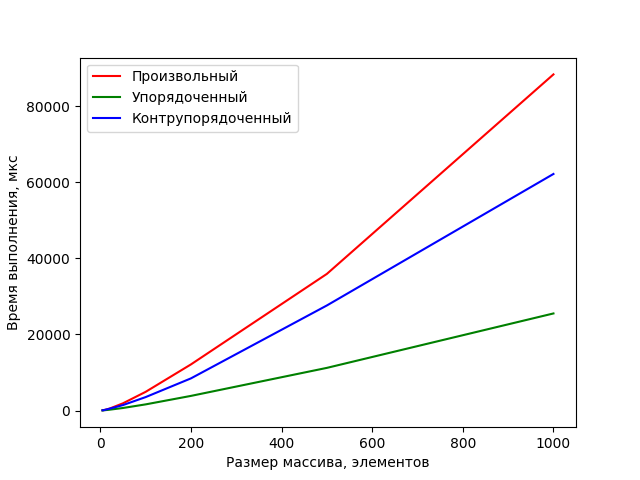
\includegraphics[width=1\linewidth]{images/shaker_graph}
	\caption{Зависимость времени работы алгоритма шейкерной сортировки от размера и упорядоченности массива}
	\label{fig:shaker_gr}
\end{figure}
\begin{figure}[H]
	\centering
	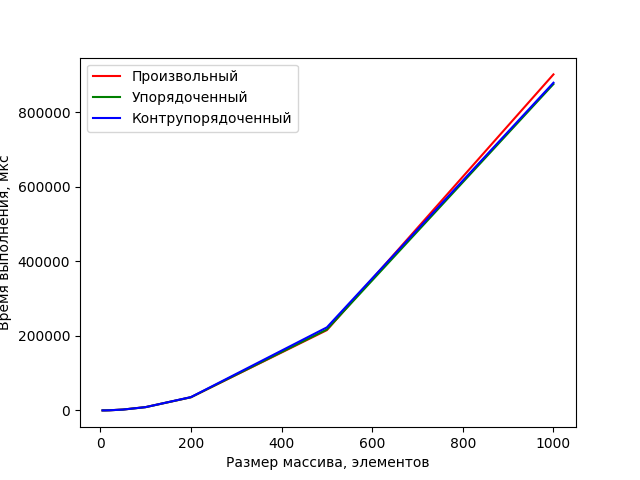
\includegraphics[width=1\linewidth]{images/selection_graph}
	\caption{Зависимость времени работы алгоритма сортировки выбором от размера и упорядоченности массива}
	\label{fig:selection_gr}
\end{figure}
\begin{figure}[H]
	\centering
	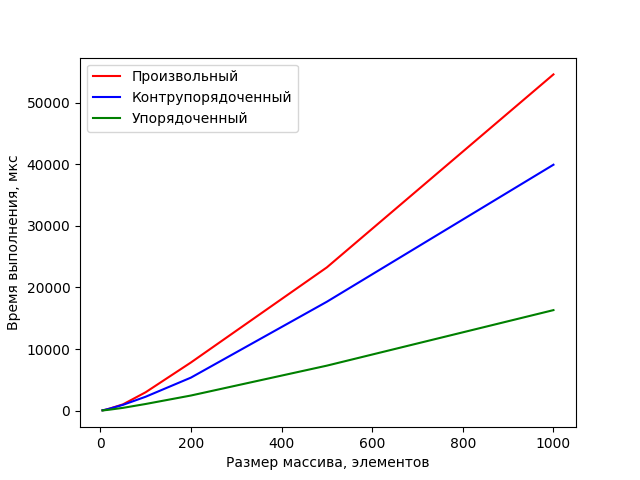
\includegraphics[width=1\linewidth]{images/shell_graph}
	\caption{Зависимость времени работы алгоритма сортировки Шелла от размера и упорядоченности массива.}
	\label{fig:shell_gr}
\end{figure}

\section{Выводы}
По результатам проведенных замеров видно, что самым быстрым является алгоритм сортировки Шелла, причем его преимущество по сравнению с сортировкой выбором составил от 1.5 до 16 раз для произвольно упорядоченных массивов, от 2 до 56 раз для отсортированных массивов и от 2 до 22 раз для отсортированных в обратном порядке; по сравнению с сортировкой перемешиванием преимущество в среднем составило от 2 до 40 раз для различно упорядоченных массивов. Время работы алгоритмов шейкерной сортировки и сортировки выбором для лучшего случая - упорядоченного массива - практически совпало с незначительным преимуществом сортировки выбором. Наименее эффективным оказался алгоритм шейкерной сортировки, проигрыш которого по сравнению с сортировкой выбором составил 2-3 раза. Худшим случаем сортировки Шелла оказался произвольно упорядоченный массив, что говорит о неподходящем выбранном шаге сравнения элементов. 
\newpage

\addcontentsline{toc}{chapter}{Заключение}
\chapter*{Заключение}
В процессе выполнения лабораторной работы были изучены и реализованы алгоритмы сортировки перемешиванием, выбором и сортировки Шелла.

Согласно проведенному анализу трудоемкости алгоритмов в соответствии с выбранной моделью вычислений, приблизительная трудоемкость шейкерной сортировки для лучшего случая равна $3n^2$, худшего - $\frac{15}{2}n^2$; сортировки выбором для лучшего случая - $\frac{5}{2}n^2$, для худшего - $3n^2$. Согласно проанализированным источникам, трудоемкость сортировки Шелла для лучшего случая равна $n \log n$, для худшего случая - $n^2$. Лучший случай для выбранных алгоритмов оказался общим, это случай обработки отсортированного массива. Худший случай совпал для шейкерной сортировки и сортировки выбором, это обработка отсортированного в обратном порядке массива. Худшим случаем для алгоритма сортировки Шелла является случай неудачного выбора шага сравнения. Таким образом, наиболее эффективной является сортировка Шелла, наименее - шейкерная сортировка.

Было исследовано процессорное время выполнения выше обозначенных алгоритмов. В результате было выявлено, что самым быстрым является алгоритм сортировки Шелла, причем его выигрыш по сравнению с сортировкой выбором составил от 1.5 до 16 раз для произвольно упорядоченных массивов, от 2 до 56 раз для отсортированных массивов и от 2 до 24 раз для отсортированных в обратном порядке; по сравнению с сортировкой перемешиванием преимущество составило от 2 до 30 раз для произвольно упорядоченных, от 2 до 56 раз для упорядоченных и от 2 до 60 раз для упорядоченных в обратном порядке массивов. Преимущество по сравнению с обоими алгоритмами увеличивается с увеличением размера массива. Время работы алгоритмов шейкерной сортировки и сортировки выбором для лучшего случая - упорядоченного массива - практически совпало с незначительным преимуществом сортировки выбором. Наименее эффективным оказался алгоритм шейкерной сортировки, проигрыш которого по сравнению с сортировкой выбором составил 2-3 раза. Худшим случаем сортировки Шелла оказался произвольно упорядоченный массив, что говорит о неподходящем выбранном шаге сравнения элементов.

Таким образом, практика подтверждает теорию, и самым эффективным является алгоритм сортировки Шелла, наименее эффективным - шейкерной сортировки.

\newpage
\addcontentsline{toc}{chapter}{Список литературы}

\bibliographystyle{utf8gost705u}
\bibliography{bib_lab_3}
\nocite{*}



\end{document}